\section{Introduction}
The recent commercial availablity of relatively cheap mobile robots such as Baxter and the UBR 1 
has created a very real possiblity for widespread application of robotics to mobile manipulation tasks.
There are huge economic gains to be had from the deployment of robotics in a variety of settings that range from homes to factories.
However, getting robots to execute complex, goal-directed tasks in such unstructured settings remains a major challenge.

Problems in these settings are characterized by state and action spaces that are high-dimensional and continuous, thereby making direct, low-level planning intractable.
In modern industrial settings, this is mitigated through intelligent design of environments and manipulation policies.
However, the time and skill required on the part of system designers prohibits application of these approaches for unstructured settings and more complex tasks.
Deformable object manipulation is an especially difficult scenario, since it is difficult to accurate model and track the underlying state of the world~\cite{SchulmanLeeHoAbbeel_ICRA2013,Javdanietal_2011,Haehnel03a}.

However, one way to mitigate these issues is to frame our problem as one of learning from demonstrations.
Rather than starting from scratch in each scenario, we generalize from a recording of an expert demonstration.
This allows us to perform our task with the guidance of a expert, thereby avoiding large unrecoverable regions of the state space.

One recent work that takes this approach uses \emph{trajectory transfer} through the use of non-rigid registration to tackle this problem.
When faced with a novel scenario, trajectory transfer fits a function $f:\mathbb{R}^3 \rightarrow \mathbb{R}^3$ that warps a demonstration scene to a novel setting.
The demonstrated trajectory is then warped with this function, and the resulting trajectory is executed in the new environment.
This has been shown to be effective for many complex tasks, including knot-tying and suturing~\cite{Schulmanetal_ISRR2013, Schulmanetal_IROS2013}.\dhm{needs several citations}

Of course, a single trajectory can only transfer to so many real-world scenarios.
Rather than relying on a single demonstration, we want to leverage a library of demonstrations and develop a method to select which trajectory to transfer.
This enables our trajectory transfer systems to perform more complex tasks by composing several expert trajectories in sequence.
However, the task of selecting a demonstration that will generalize well to the test environment is nontrivial.
Certain trajectories adapt to new settings better than others, and particular sequences of trajectories may perform tasks more efficiently than others.
Na\"{\i}ve approaches that simply use the goodness of the warping fit discard much of this information and often fail to accomplish tasks that would be possible with a different sequence of trajectories.

\begin{figure}[t]
  \centering
    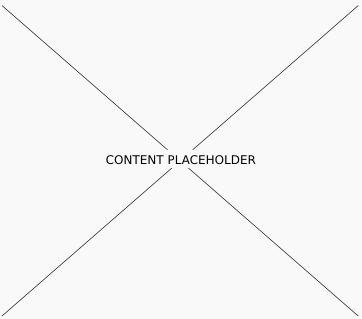
\includegraphics[width=0.9\linewidth]{figures/placeholder.png}
  \caption{Cute picture of robot tying knot}
  \label{fig:frontfig}
\end{figure}

In this paper, we present a solution to the demonstration selection problem that can account for the variability in robustness of demonstrations and the sequential nature of our tasks.
Given a set of demonstrations and a method for applying them to similar situations, we construct a discrete action abstract Markov decision process (MDP).
Each action in this MDP is associated with a demonstration, and our transition function is defined as applying trajectory transfer to generalize that demonstration.

We use the optimality of the expert-provided examples and the temporal constraints imposed by the sequential nature of our tasks to form a max-margin optimization problem.
Our objective is a linear combination of features which are completely task-agnostic and can be applied to any problem where trajectory transfer is appropriate. 
Solving this problem allows us to learn a $Q$-function from these example sequences of state-demonstration pairs, which in turn enables us to determine demonstration selection policies that effectively accomplish the task at hand.
We investigate the utility of this approach in a knot-tying scenario and show that the greedy application of our learned policy outperforms the nearest-neighbor baseline on a challenging distribution of problems. 
We also leverage the additional structure of the $Q$-function over a direct policy to look ahead to future states, enabling near-perfect performance in this setting.
Finally, we present a method for bootstrapping, though a process we call leave-one-out labeling, that enables us to do max-margin $Q$-learning with no additional human supervision beyond the initial demonstrations.

The rest of this paper is organized as follows: first, we review related work in
the field and discuss what differentiates our method. Next, we provide relevant
technical background for our method. We then provide a formal formulation of the
trajectory selection problem as a max-margin Q-learning problem, as well as a
discussion of the various features and policies that can be used with this
framework. We present experimental results in a knot-tying setting and provide
results that show that our learned policy can successfully tie a knot
significantly more often than the na\"{\i}ve nearest-neighbor approach. Finally,
we conclude with a summary of our work and a discussion of future work.
